\documentclass[conference]{IEEEtran}
\IEEEoverridecommandlockouts

\usepackage{cite}
\usepackage{amsmath,amssymb,amsfonts}
\usepackage{algorithmic}
\usepackage{algorithm}
\usepackage{graphicx}
\usepackage{textcomp}
\usepackage{xcolor}
\usepackage{booktabs}
\usepackage{hyperref}
\usepackage{array}

% Path to extracted images folder
\graphicspath{{images/}}

\def\BibTeX{{\rm B\kern-.05em{\sc i\kern-.025em b}\kern-.08em
    T\kern-.1667em\lower.7ex\hbox{E}\kern-.125emX}}

\begin{document}

\title{Resilient Routing in Wireless Mesh Networks using Digital Twin and GNN-Based Reinforcement Learning}

\author{
  \IEEEauthorblockN{Anandakrishnan K V, Drupad M D}
  \IEEEauthorblockA{
    \textit{Department of Computer Science and IT,}\\
    \textit{School of Computing,}\\
    \textit{Amrita Vishwa Vidyapeetham,}\\
    \textit{Kochi, Kerala, India}
  }
}

\maketitle

%------------------------------------------------------------------
\begin{abstract}
A Wireless Mesh Network (WMN) is a communications network made up of multiple radio nodes organized in a mesh topology used for connecting dynamically with each other. Their flexibility in dynamic connectivity and multi-hop capabilities can attract major threats. Particularly, jamming attacks can severely degrade network performance by disrupting routing and data transmission. Traditional routing protocols lack the adaptability to operate effectively in such dynamic and hostile environments. This article proposes an integrated resilience framework for WMNs that combines digital twin modelling, graph neural networks, and reinforcement learning. A digital twin simulates realistic network behaviour and jamming scenarios, while a GAT model captures the topological and traffic features. A multi-agent deep Q-network utilizes these embeddings to learn adaptive routing strategies under varying jamming conditions.
\end{abstract}

\begin{IEEEkeywords}
Digital twin, routing, jamming detection, DQN, GNN.
\end{IEEEkeywords}

%------------------------------------------------------------------
\section{Introduction}

Wireless communication networks have greatly influenced the advancement of interconnectivity of the technology without a physical medium. The main problem is that the reach of a single wireless device is far too limited for proper networking. This is where Wireless Mesh Networks (WMNs) fill the gap. WMNs use multi-hop routing to extend the coverage of data transmission. Multiple nodes are interconnected and take part in a single information transfer. Having a decentralized architecture makes them handy in real-world applications like disaster response, industrial automation, and Internet of Things (IoT). Due to this flexibility, WMNs are also prone to different kinds of attacks. These attacks damage the interconnectivity of the nodes, affect network reliability, delay sensitive communication, and affect overall Quality-of-Service (QoS).

Conventional methods for network resilience, including heuristic-based topology control and rule-based routing, fall short in dynamic environments, while mathematical optimization approaches face scalability limitations. Reinforcement Learning (RL) techniques have shown promise in adaptive, real-time decision-making in dynamic environments. However, many such methods still rely on centralized architectures that degrade the decentralized nature of WMNs.

To mitigate these problems, this paper proposes a novel approach that integrates three technologies: a Digital Twin (DT), Multi-Agent Deep Q-Networks (DQN), and a Graph Attention Network (GAT). Together, these form the basis for jamming detection and fault tolerance in resilient WMNs.

\begin{itemize}
  \item \textbf{Digital Twin (DT):} A real-time virtual mirror of the real network that enables detection of anomalies and analysis of predictive failures. By comparing actual and expected radio signals, the DT can detect jamming attacks and analyze their impacts.
  \item \textbf{Multi-Agent DQN:} Extends traditional RL by enabling nodes to collaboratively adapt their routing and transmission policies. Each node has an embedded agent that learns to optimize local and global performance using its own policy network while sharing experiences across agents.
  \item \textbf{Graph Attention Network (GAT):} An attention-based Graph Neural Network (GNN) framework used to extract structural features from the network graph. By aggregating information from neighbouring nodes through learned attention weights, GATs generate node embeddings that guide routing decisions and facilitate anomaly detection.
\end{itemize}

In short, these components together can detect and mitigate threats and adapt to changing network conditions, forming the basis for a scalable and dynamic routing solution for WMNs.

%------------------------------------------------------------------
\section{Related Work}

Recent developments in wireless mesh networks show a clear shift from fixed rule-based protocols to dynamic machine learning-driven techniques. This evolution is driven by the increasing complexity of network dynamics, including challenges such as node mobility, spectral interference, and fluctuating traffic loads.

\subsection{Reinforcement Learning and Graph Neural Networks in Routing}

Routing in WMNs is typically modeled as a Markov Decision Process (MDP), allowing autonomous agents to develop optimal routing policies by exploring and interacting with their environment.

\textbf{Deep Reinforcement Learning (DRL) and GNNs:}
Pappone et al.~\cite{pappone2023} proposed a framework that integrates GNNs with Multi-Agent Deep Reinforcement Learning (DRL) to overcome a core limitation of traditional RL: the inability to generalize to unfamiliar network topologies without significant retraining. By encoding the network state using GNNs, their model captures the graph's permutation-invariant structure, enabling agents to minimize flow collisions and adapt to real-time topology changes dynamically.

Similarly, Jin et al.~\cite{jin2025} researched a Deep Reinforcement Learning-based Resilient Routing (DRLRR) approach for urban emergency communication networks. To counter the overestimation bias of conventional Q-learning, they used Double Deep Q-Networks (DDQN), enabling stable route optimization despite excessive node degradation scenarios.

\textbf{Graph Convolutional Networks (GCN):}
GCNs gained popularity in 2017 thanks to Kipf and Welling~\cite{kipf2017}. The objective was to enable models to learn on graphs using an efficient spectral approximation of convolution. In this approach, each node's representation is iteratively refined by aggregating the features of its local neighbours, normalized by the degrees of related nodes. Formally, the GCN layer-wise propagation rule is:

\begin{equation}
  H^{(l+1)} = \sigma\!\left(\tilde{D}^{-\frac{1}{2}}\tilde{A}\,\tilde{D}^{-\frac{1}{2}} H^{(l)} W^{(l)}\right)
  \label{eq:gcn}
\end{equation}

\noindent where:
\begin{itemize}
  \item $\tilde{A} = A + I_N$ is the adjacency matrix with added self-connections,
  \item $\tilde{D}$ is the degree matrix of $\tilde{A}$,
  \item $W^{(l)}$ is the layer-specific trainable weight matrix, and
  \item $\sigma$ is the activation function (e.g., ReLU).
\end{itemize}

\textbf{Graph Attention Network (GAT):}
In 2018, Veli\v{c}kovi\'{c} et al.~\cite{velickovic2018} introduced GAT, which features a self-attention mechanism that computes attention coefficients $\alpha_{ij}$ indicating how important neighbour $j$ is to node $i$:

\begin{equation}
  \alpha_{ij} = \frac{
    \exp\!\left(\mathrm{LeakyReLU}\!\left(\mathbf{a}^T \left[\mathbf{W}\vec{h}_i \,\|\, \mathbf{W}\vec{h}_j\right]\right)\right)
  }{
    \displaystyle\sum_{k \in \mathcal{N}_i} \exp\!\left(\mathrm{LeakyReLU}\!\left(\mathbf{a}^T \left[\mathbf{W}\vec{h}_i \,\|\, \mathbf{W}\vec{h}_k\right]\right)\right)
  }
  \label{eq:gat}
\end{equation}

Unlike GCN, which assigns uniform weights during aggregation, GAT selectively weights each neighbour's contribution through a learnable attention mechanism. This makes it particularly suited for environments where link reliability varies due to jamming or interference. Selective aggregation allows GAT to better capture the importance of high-quality, non-jammed links during routing, which is the core motivation for its adoption in this framework.

\subsection{Fault and Anomaly Detection}

Understanding the present condition of the network has a direct impact on routing performance. It is important to determine whether a disruption is the consequence of a routine malfunction or something more intentional before making routing decisions.

\textbf{Digital Twin for Radio Environments:}
Krause et al.~\cite{krause2023} proposed a rethinking of anomaly detection in radio environments. Rather than anchoring detection to patterns mined from past data, their system maintains a physics-based virtual replica of the network running in real time. A ray-tracing engine inside the replica computes expected RSSI readings across each link under normal conditions. Any meaningful gap between predicted and measured signals is flagged—no attack examples are needed for training. Crucially, the framework distinguishes jamming from ordinary fading, which is exactly where conventional statistical detection tends to fail.

\subsection{Gap Analysis}

Pappone et al.~\cite{pappone2023} built a solid routing foundation, yet the work overlooks the subtleties of physical-layer threats by anchoring itself to standard network metrics. Krause et al.~\cite{krause2023} take a different angle leveraging digital twins for detection but deliberately stop at observation, leaving the door closed on any form of active network intervention.

Existing work has yet to meaningfully explore the tight integration of these two systems—particularly the idea of feeding high-fidelity anomaly scores from a Digital Twin directly into a GAT as live, dynamic features. This paper steps into that gap. The core proposition is that routing the Digital Twin's ground-truth awareness through the attention mechanism of a GAT-based RL agent enables the network to build genuine resilience: one where interference is anticipated and routed around before packet loss has a chance to escalate.

%------------------------------------------------------------------
\section{Proposed Framework}

\subsection{Digital Twin}

This framework is grounded in a Digital Twin (DT) implemented through a Mesh Digital-Twin module. Unlike conventional routing mechanisms that depend on packet-level feedback, the Digital Twin maintains a virtual copy of the physical network that is continuously updated.

\textbf{Radio Map:}
The Digital Twin ingests environmental radio maps containing Received Signal Strength (RSS) measurements, which are linked to link-level performance indicators including latency and bandwidth capacity. Sigmoidal transformation functions convert RSS values into estimates, allowing the model to capture non-linear signal propagation effects and represent real-time variations in channel conditions and interference.

\textbf{Feature Enrichment and Anomaly Awareness:}
To enhance environmental awareness, the DT employs anomaly detection and jamming analysis modules (\texttt{AnomalyBridge} and \texttt{JammerDetector}). These components augment the network graph by incorporating additional information into each node's representation. Each node is described by a seven-dimensional feature vector consisting of: average latency, average bandwidth, anomaly scores, estimated jamming probability, average jamming intensity, and routing role indicators. These features give the agent a comprehensive understanding of both the network state and the environmental challenges it may face.

\subsection{Graph Attention Networks}

The decision-making core of the proposed framework is a Graph Attention Network (GAT), used to embed the entire network topology and the dependencies between each node.

\textbf{Input Representation:}
The seven-dimensional feature vector described in Section~\ref{sec:dt-features} is provided as input to the GAT. The graph-based formulation enables the model to learn about both topographical and environmental information simultaneously.

\textbf{Message Passing:}
Information is propagated between neighbouring nodes through two GAT layers. Using learned attention weights, nodes selectively focus on important neighbours based on their relevance to routing, enabling the propagation of information about node failures or jamming attacks across the network.

\textbf{Q-Value Estimation:}
The output embeddings generated by the attention layers are passed through fully connected layers to estimate Q-values. Each Q-value denotes the expected reward from selecting a neighbour as the next hop. Routing decisions are framed as discrete actions, each yielding a corresponding reward.

\subsection{Deep Q-Network Learning}

The learning process is based on the Deep Q-Network (DQN) architecture adapted for graph-like environments such as mesh networks. The agent combines GAT's state representations with RL techniques as follows.

\textbf{Experience Replay:}
During training, interaction tuples $(s, a, r, s')$ are stored in a replay memory. Mini-batches are randomly sampled from this memory, reducing temporal correlations between training samples and improving convergence stability.

\textbf{Exploration Strategy:}
The framework uses an epsilon-greedy policy to balance exploration and exploitation. In the early stages of training, the agent explores the environment broadly; the exploration rate $\varepsilon$ then decays gradually so that the agent increasingly relies on learned policies.

\subsection{Reward Function}
\label{sec:reward}

The reward function is designed to promote efficient routing and minimize detours.

\textbf{Base Reward:}
The base reward is calculated according to the agent's progress towards the destination, promoting a fewer-hops, greater-reward policy.

\textbf{Anomaly Penalization:}
The agent is penalized for routing through unstable nodes. The anomaly dampening factor is defined as:
\begin{equation}
  r_{\text{anomaly}} = -\lambda \cdot s_{\text{anomaly}}
  \label{eq:anomaly}
\end{equation}
where $\lambda$ controls the impact of detected anomalies. Nodes exhibiting abnormal behaviour receive reduced rewards.

\textbf{Jamming Penalty:}
A negative reward is applied when the agent selects a node identified as jammed, discouraging routing through highly interfered regions.

\textbf{Resilience Incentive:}
An additional reward is granted upon successful completion of routing, reinforcing the importance of end-to-end delivery and making the network resilient in nature.

\begin{algorithm}[htbp]
\caption{Resilient Routing with MA DT-GCN}
\label{alg:madtgcn}
\begin{algorithmic}[1]
\STATE \textbf{Initialize} DT radio map, MA-DQN agent replay buffers $B_i$, and GAT networks with arbitrary weights.
\FOR{each training episode}
    \STATE \textbf{Reset} network topology and initialize each packet at source nodes.
    \WHILE{packet not at destination and max steps not reached}
        \STATE \textbf{Digital Twin Update:} Retrieve real-time RSS map and compute anomaly/jamming probabilities.
        \STATE \textbf{State Representation:} For each node $i$, construct the 7-dimensional feature vector $\mathbf{x}_i$.
        \STATE \textbf{GAT Attention:} Compute node embeddings $\vec{h}_i$ by aggregating neighbour information using learned attention coefficients $\alpha_{ij}$ (Eq.~\ref{eq:gat}).
        \FOR{each agent $i$ with a packet}
            \STATE \textbf{Action Selection:} With probability $\varepsilon$ select a random neighbour $a_t$; otherwise select $a_t = \arg\max_{a} Q(\vec{h}_i, a; \theta_i)$.
            \STATE \textbf{Execute} action $a_t$ (forward packet to neighbour $a_t$).
            \STATE \textbf{Observe} reward $r_t$ (progress, anomaly penalty, jamming penalty) and next state embeddings $\vec{h}'_i$.
            \STATE \textbf{Store} transition $(\vec{h}_i, a_t, r_t, \vec{h}'_i)$ in replay buffer $B_i$.
        \ENDFOR
        \STATE \textbf{Experience Replay:} Sample mini-batches from $\bigcup_i B_i$.
        \STATE \textbf{Policy Update:} Perform gradient descent on DQN loss to update network weights $\theta_i$.
    \ENDWHILE
    \STATE Decay exploration rate $\varepsilon$.
\ENDFOR
\end{algorithmic}
\end{algorithm}

%------------------------------------------------------------------
\section{Experiments and Results}

\subsection{Experimental Setup}

To evaluate the proposed MA DT-GCN routing protocol, a comparative analysis was conducted between the MA DT-GCN and a GAT-based routing baseline on a 50-node wireless mesh network over 3,000 training episodes. Two models were compared:

\begin{enumerate}
  \item \textbf{GAT Baseline (4 Features):} A single-agent GAT model utilizing basic node information — routing state (source/destination flags) and link quality (latency and bandwidth) — without cooperative agent interactions or Digital Twin features.
  \item \textbf{MA DT-GCN (7 Features):} The proposed model augments the baseline feature set with three DT-derived parameters: anomaly score, jamming probability, and neighbour jamming average.
\end{enumerate}

To ensure fairness, both models were tested over 3,000 episodes on the same network. Four key metrics were monitored: average reward, average path length (hop count), average success rate (packet delivery ratio), and average number of jammed steps per episode.

\begin{figure}[htbp]
  \centering
  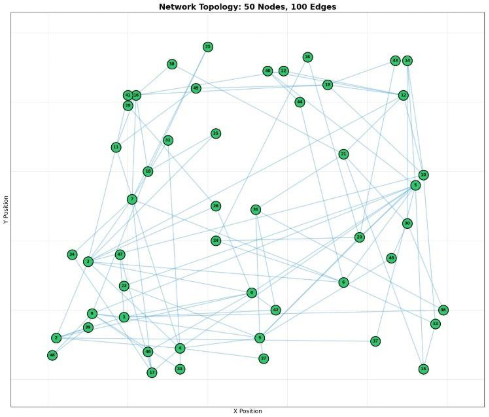
\includegraphics[width=\linewidth]{image.png}
  \caption{Simulated WMN topology: 50 nodes and 100 edges used as the experimental testbed.}
  \label{fig:topology}
\end{figure}

\subsection{Performance Analysis}

The results demonstrate that the Multi-Agent DT-GCN model outperforms the GAT baseline across all measured metrics. An overview of the comparative performance is provided in Table~\ref{tab:performance}.

\begin{table}[htbp]
  \centering
  \caption{Comparative Performance Metrics (3,000 Episodes)}
  \label{tab:performance}
  \begin{tabular}{lcc}
    \toprule
    \textbf{Metric} & \textbf{GAT Baseline} & \textbf{MA DT-GCN} \\
    \midrule
    Average Reward          & $-12.452$ & $-2.435$  \\
    Avg.\ Path Length (hops) & $34.71$   & $11.01$   \\
    Success Rate (\%)        & $95\%$    & $96\%$    \\
    Avg.\ Jammed Steps       & $2.72$    & $1.15$    \\
    Training Time (min)      & $75.2$    & $35.5$    \\
    \bottomrule
  \end{tabular}
\end{table}

\subsubsection{Reward and Routing Stability}

The MA DT-GCN achieved an average reward of $-2.435$ compared to the baseline's $-12.452$. This significant improvement demonstrates the effectiveness of the Digital Twin model in minimizing interference, reducing path costs, and lowering the cost of unsuccessful transmissions. The knowledge shared among 50 cooperative agents allowed the MA DT-GCN to avoid high-penalty zones that the baseline, lacking awareness of network dynamics, frequently traversed.

\begin{figure}[htbp]
  \centering
  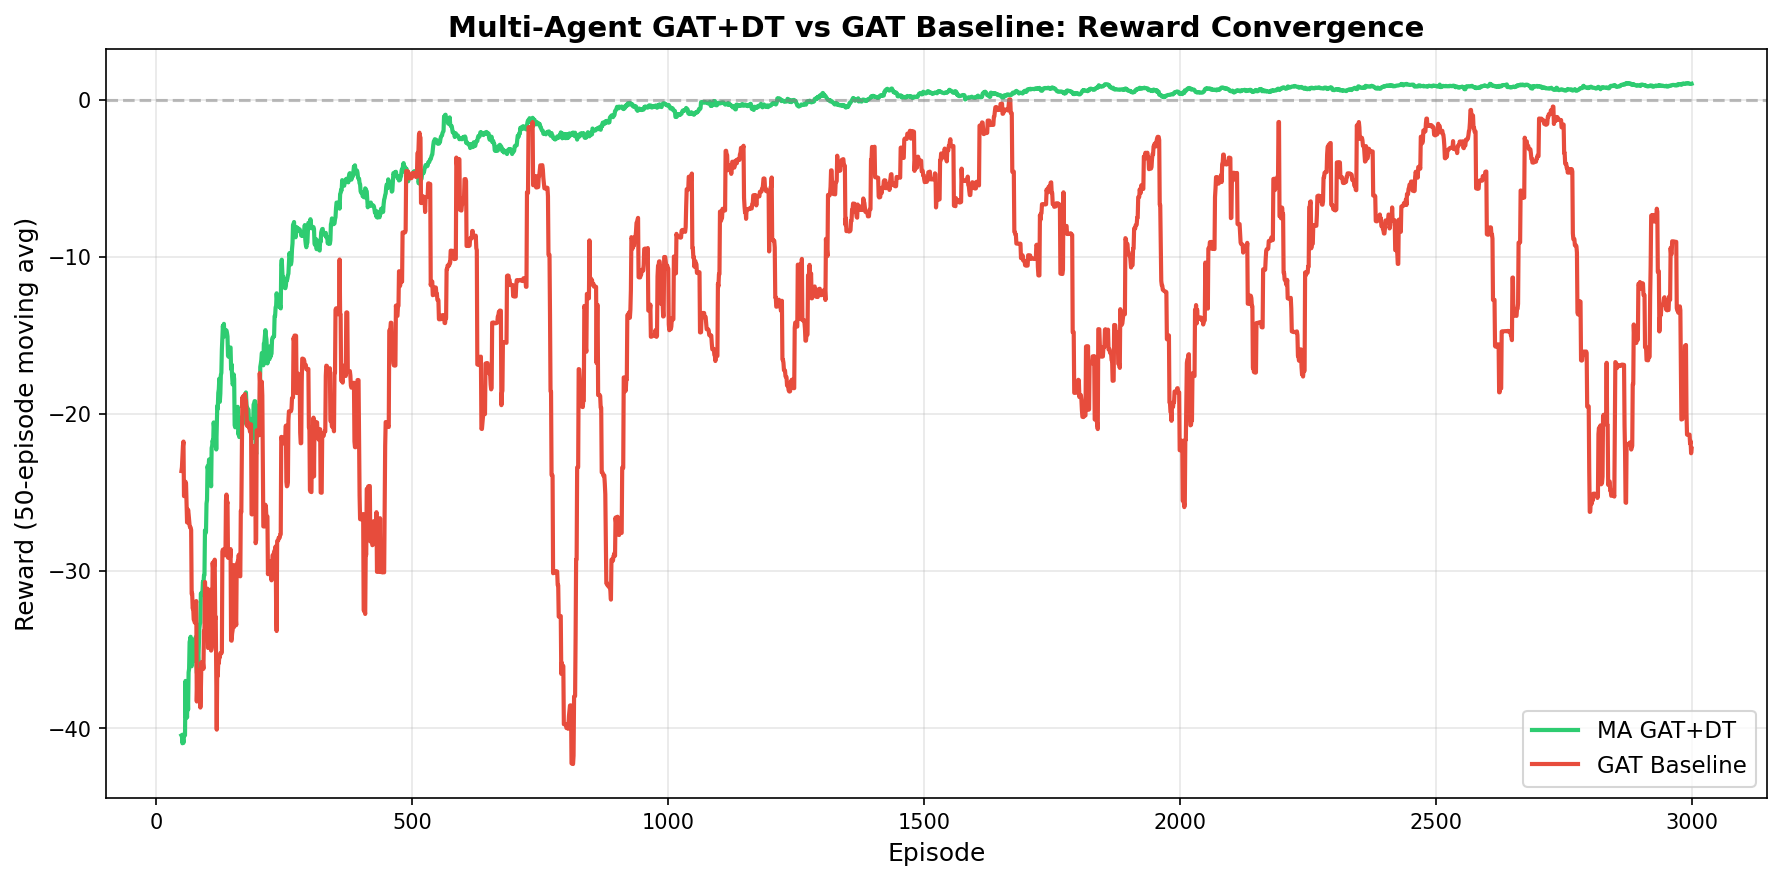
\includegraphics[width=\linewidth]{image5.png}
  \caption{Reward convergence over 3,000 episodes: MA GAT+DT (green) vs.\ GAT Baseline (red), 50-episode moving average.}
  \label{fig:reward}
\end{figure}

\subsubsection{Path Efficiency and End-to-End Latency}

The MA DT-GCN achieved an average path length of 11.01 hops, compared to 34.71 hops for the GAT baseline—a reduction of 23.70 hops per episode on average. Cooperative agents leveraging DT features (jamming probability and anomaly scores) identified shorter paths, reducing the number of relay nodes, queuing time, and probability of packet loss. The 50 cooperative agents in the MA DT-GCN effectively avoided overloaded nodes, enabling efficient traffic delivery.

\subsubsection{Jamming Avoidance and Network Robustness}

The MA DT-GCN reduced average jammed steps from 2.72 to 1.15, corresponding to a reduction of 57.7\%. This demonstrates the effectiveness of incorporating real-time DT jamming information into the routing decision process. The ability of 50 cooperative agents to jointly identify and avoid jammed nodes validates the proposed framework's robustness under adversarial conditions.

\begin{figure}[htbp]
  \centering
  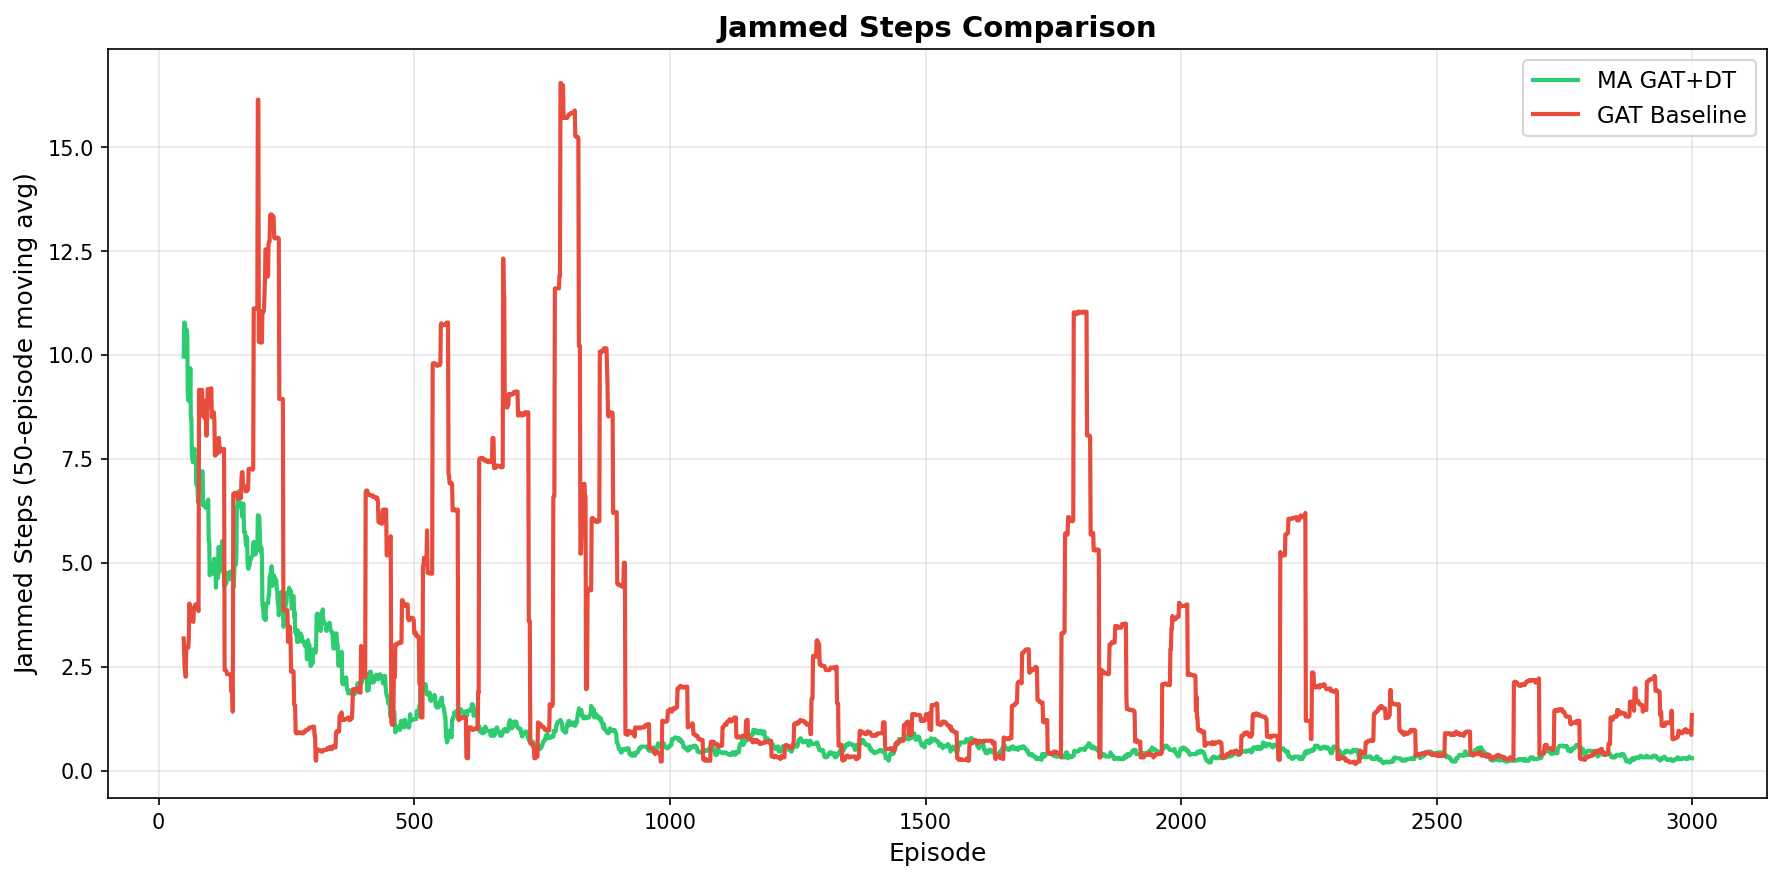
\includegraphics[width=\linewidth]{image6.png}
  \caption{Jammed steps comparison over 3,000 episodes: MA GAT+DT maintains near-zero jammed steps while the GAT Baseline shows persistent interference exposure.}
  \label{fig:jammed}
\end{figure}

\subsubsection{Convergence Behaviour and Training Efficiency}

The MA DT-GCN completed 3,000 training episodes in 35.5 minutes, compared to 75.2 minutes for the GAT baseline—a speedup of 52.8\%. This improvement is notable given that the MA DT-GCN coordinates 50 agents simultaneously, each with its own policy network. The shared experience replay mechanism enabled agents to explore the state space more thoroughly in parallel, accelerating policy learning relative to the single-agent baseline.

\begin{figure}[htbp]
  \centering
  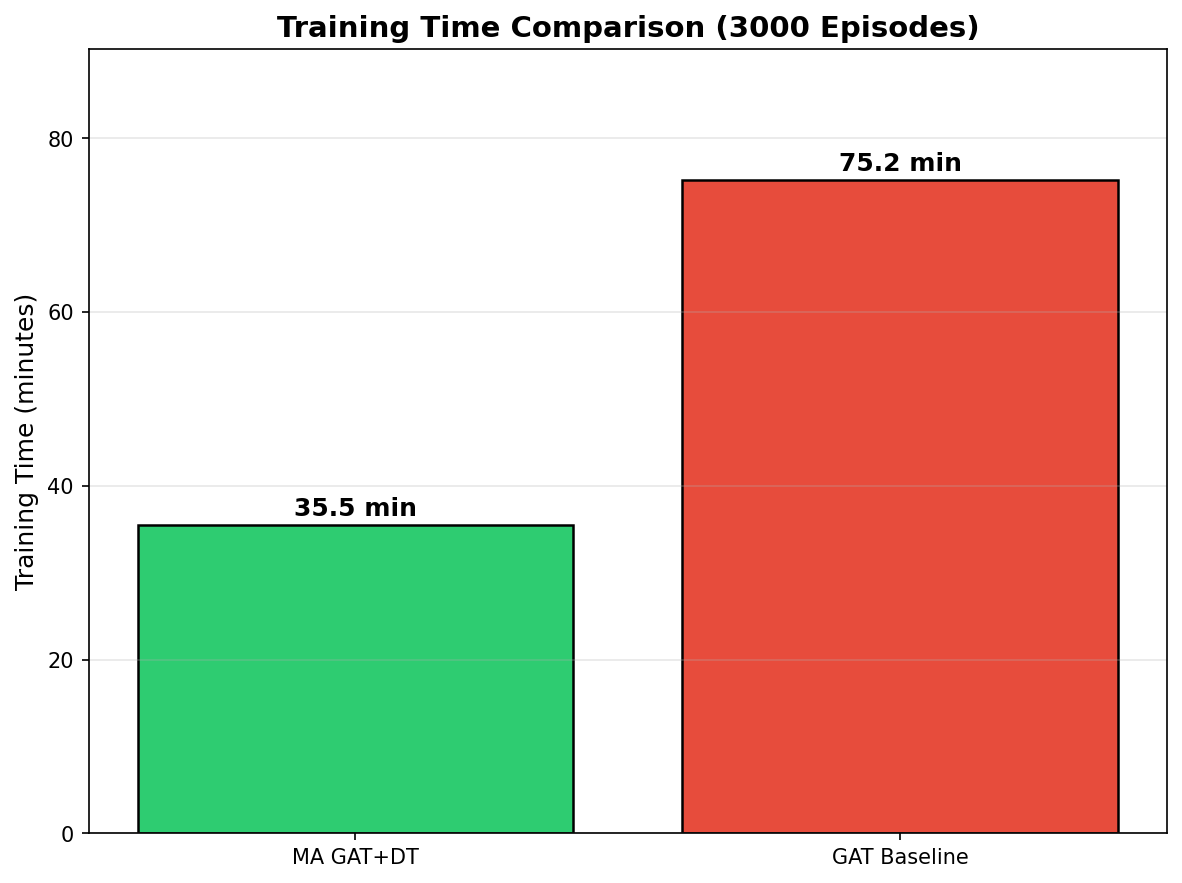
\includegraphics[width=0.85\linewidth]{image8.png}
  \caption{Training time comparison for 3,000 episodes: MA GAT+DT (35.5 min) vs.\ GAT Baseline (75.2 min).}
  \label{fig:training_time}
\end{figure}

\subsubsection{Success Rate and Reliability}

The MA DT-GCN achieved a success rate of 96\% over 3,000 episodes, compared to the baseline's 95\%. More importantly, the quality of the routes generated was substantially superior: the MA DT-GCN produced routes averaging 11.01 hops and an average reward of $-2.435$, versus the baseline's 34.71 hops and average reward of $-12.452$.

\begin{figure}[htbp]
  \centering
  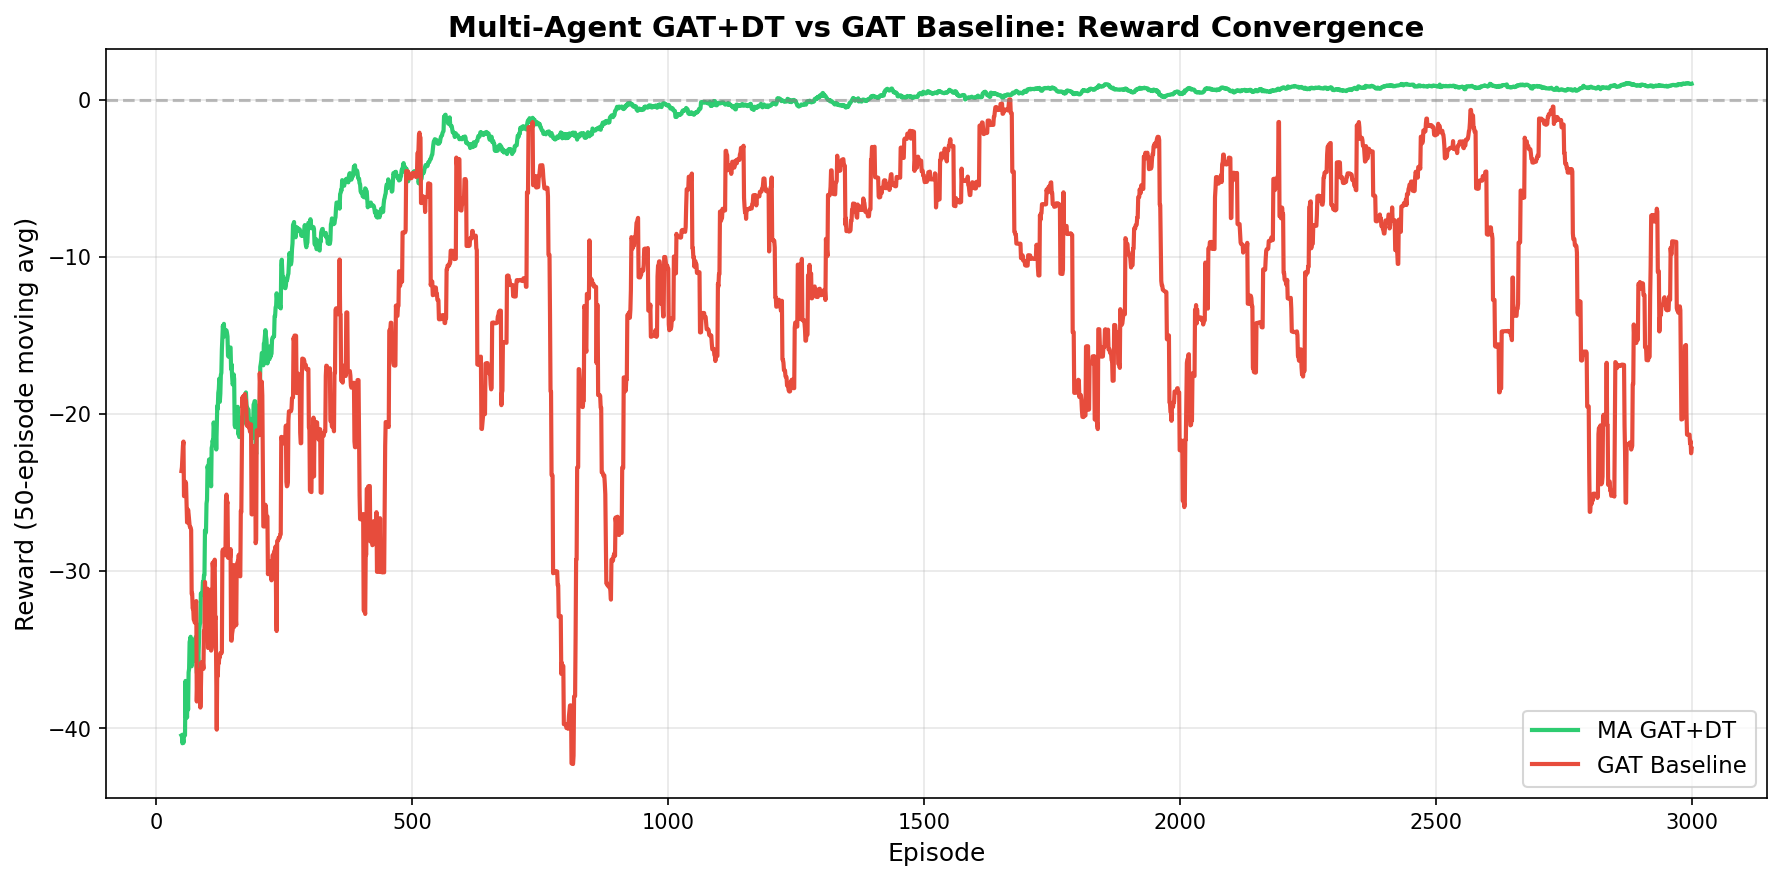
\includegraphics[width=\linewidth]{image7.png}
  \caption{Reward convergence comparison highlighting consistent MA GAT+DT superiority in route quality across all 3,000 training episodes.}
  \label{fig:reward2}
\end{figure}

The baseline's inferior performance stems from its lack of awareness of jamming signals and anomalies, leading to longer, exposed routes prone to interference. The MA DT-GCN, equipped with shared knowledge from 50 cooperative agents and Digital Twin information, consistently made better routing decisions across all performance indicators.

%------------------------------------------------------------------
\section{Conclusion}

This paper proposes an integrated resilience architecture that leverages Digital Twin modelling, Graph Attention Networks, and Multi-Agent Deep Q-Networks for adaptive, jamming-aware routing in Wireless Mesh Networks. The proposed MA DT-GCN model significantly outperformed the GAT baseline across 3,000 training episodes while converging 52.8\% faster.

Future work may explore integrating transfer learning to enable the trained MA DT-GCN model to generalize across multiple wireless mesh topologies without retraining from scratch. Furthermore, deploying this framework on real hardware testbeds with live radio interference would validate the Digital Twin's accuracy and practical usefulness beyond simulation.

%------------------------------------------------------------------
\begin{thebibliography}{00}

\bibitem{pappone2023}
A.~Pappone \textit{et al.}, ``Graph Neural Network and Multi-Agent Deep Reinforcement Learning for Adaptive Routing in Wireless Mesh Networks,'' 2023.

\bibitem{jin2025}
Z.~Jin \textit{et al.}, ``Deep Reinforcement Learning-Based Resilient Routing for Urban Emergency Communication Networks,'' 2025.

\bibitem{kipf2017}
T.~N.~Kipf and M.~Welling, ``Semi-Supervised Classification with Graph Convolutional Networks,'' in \textit{Proc. ICLR}, 2017.

\bibitem{velickovic2018}
P.~Veli\v{c}kovi\'{c} \textit{et al.}, ``Graph Attention Networks,'' in \textit{Proc. ICLR}, 2018.

\bibitem{krause2023}
R.~Krause \textit{et al.}, ``Digital Twin-Based Anomaly Detection in Radio Environments,'' 2023.

\end{thebibliography}

\end{document}
